\problemname{Planetbacke}

I en inte alltför avlägsen framtid har forskare upptäckt inte bara {\em en} tidigare okänd planet här i vårt egna solsystem (se uppgiften Planet X) utan nu {\em ytterligare en}, kallad planet Y.

Forskarna är intresserade av hur topografin på Planet Y ser ut, och har lyckats mäta detta med stor noggrannhet. Vi representerar ytan som ett $N \times M$ rutnät, där varje ruta har en uppmätt höjd mellan 0 och 9.

Till mångas glädje visar det sig att planet Y har perfekt klimat för skidåkning (som du säkert förstår finns det inte längre någon snö på jorden vid det här laget). Skriv ett program som beräknar den längsta skidbacke som kan byggas på planet Y.

Kravet på en skidbacke är att det ska vara en sammanhängande sekvens av rutor där varje par av rutor gränsar till varandra antingen via en gemensam sida eller ett gemensamt hörn (se figurerna nedan), och där varje ruta i sekvensen inte har högre höjd än den föregående. Det är alltså i princip tillåtet att alla rutor i skidbacken har samma höjd. Samma ruta får inte användas flera gånger men skidbacken skulle ändå kunna korsa sig själv genom ett hörn som i det andra exemplet nedan.

\section*{Indata}
På den första raden står två heltal $1 \le N,M \le 7$, 
antalet rader och kolumner i rutnätet.
Därefter följer $N$ rader med $M$ tecken på varje.
Det $j:te$ tecknet på rad $i$ är en siffra mellan
0 och 9 som motsvarar höjden för rutan. Det finns aldrig fler än $7$ rutor i rutnätet som har samma höjd.

\section*{Utdata}
Programmet ska skriva ut ett heltal: det största antalet rutor som kan ingå i en godkänd skidbacke.

\section*{Poängsättning}

För testfall värda $20$ poäng gäller att $1\leq M,N \leq 3$. \\
För testfall värda ytterligare $20$ poäng gäller att inga angränsande rutor har samma höjd. \\
För testfall värda ytterligare $20$ poäng gäller att varje ruta gränsar till högst två rutor med samma höjd som sig själv.\\

\begin{figure}[h]
  \centering
      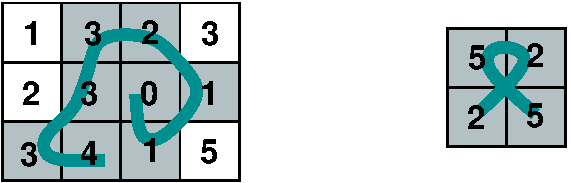
\includegraphics[width=0.7\textwidth]{planetbackefig2}
      \caption{Till vänster visas första exemplet och till höger det andra exemplet. Det tjocka strecket visar skidbackens sträckning och de skuggade rutorna är de rutor som ingår i skidbacken.}
\end{figure}
